% ||||||||||||||||||||||||||||||||||||||||||||||
% Capitulo de Revisão Bibliográfica
% ||||||||||||||||||||||||||||||||||||||||||||||

\chapter{Revisão Bibliográfica}

Fazer:
\begin{itemize}
    \item Conceito básico de máquinas rotativas
    \item Conceito de MOtor Elétricos
    \item Falar de motores elétricos CC e, por último, sobre Indução, fazendo o link com a próxima etapa
\end{itemize}

%++++++++++++++++++++++++++++++++++++++++++++++++++++++++++++++++
% 
%++++++++++++++++++++++++++++++++++++++++++++++++++++++++++++++++

\section{Motores Elétricos de Indução}\label{sec:}

Fazer:
\begin{itemize}
    \item conceitos gerais usando Fitzgerald
    \item Rotor
    \item Estator
    \item Buscar algo sobre corrente elétrica ou complementar em relação ao circuito equivalente
\end{itemize}

\begin{figure}[H]
    \caption{.}
    \begin{center}
        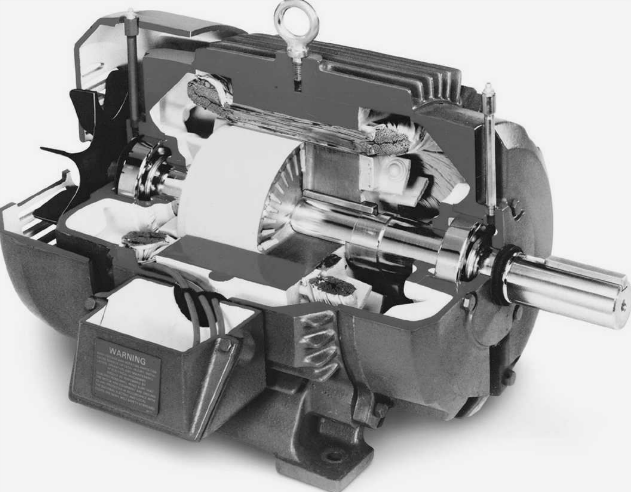
\includegraphics[scale=.45]{referencial/img/motor_fitzgerald_p345.png}
    \end{center}
    \fonte{.} 
    \label{fig:}
\end{figure}


\begin{figure}[H]
    \caption{.}
    \begin{center}
        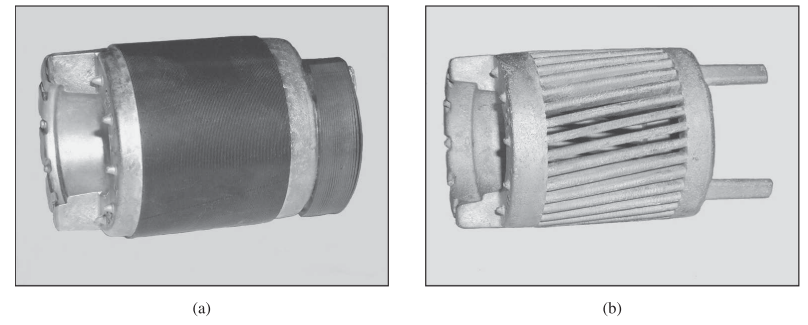
\includegraphics[scale=.5]{referencial/img/rotor_fitzgerald_p345.png}
    \end{center}
    \fonte{.} 
    \label{fig:}
\end{figure}


\begin{figure}[H]
    \caption{.}
    \begin{center}
        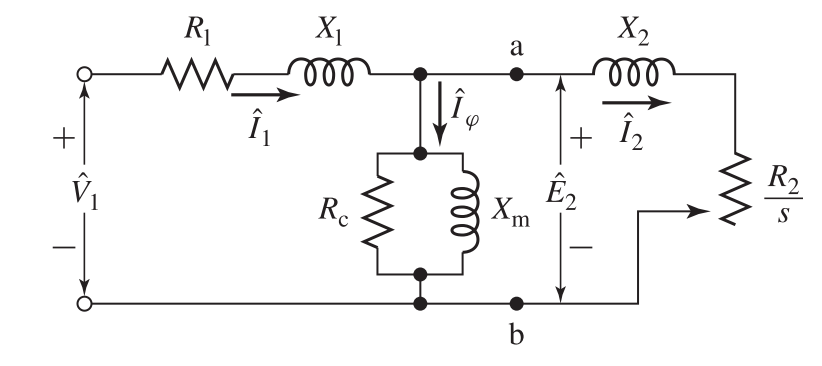
\includegraphics[scale=.35]{referencial/img/circuit_fitzgerald_p354.png}
    \end{center}
    \fonte{.} 
    \label{fig:}
\end{figure}

%----------------------------------------------------------------
% 
%----------------------------------------------------------------

\section{Falhas em Motores Elétricos de Indução}\label{sec:}

Fazer:
\begin{itemize}
    \item Conceitos básicos e a importância das falhas
    \item Listar as principais falhas e lincar com os efeitos
    \item explicar a imagem sobre todos os tipos de falhas e elencar as mais comuns via refêrencia
    \item após a etapa acima, apresentar os principais problemas de acordo com as imagens
\end{itemize}

\begin{figure}[H]
    \caption{.}
    \begin{center}
        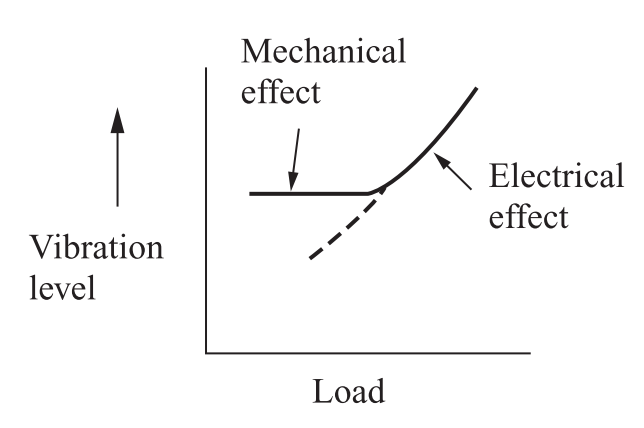
\includegraphics[scale=.45]{referencial/img/fault_effect_randall_p54.png}
    \end{center}
    \fonte{.} 
    \label{fig:}
\end{figure}


\begin{figure}[H]
    \caption{.}
    \begin{center}
        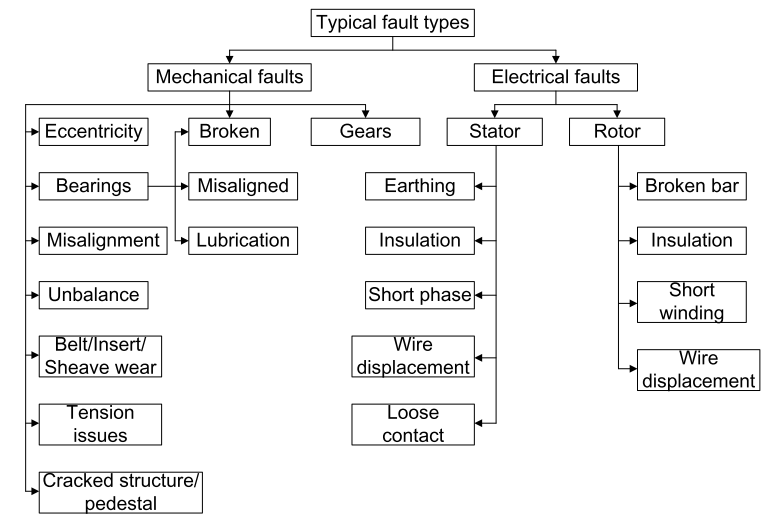
\includegraphics[scale=.5]{referencial/img/faults_rilski_p77.png}
    \end{center}
    \fonte{.} 
    \label{fig:}
\end{figure}


\begin{figure}[H]
    \caption{.}
    \begin{center}
        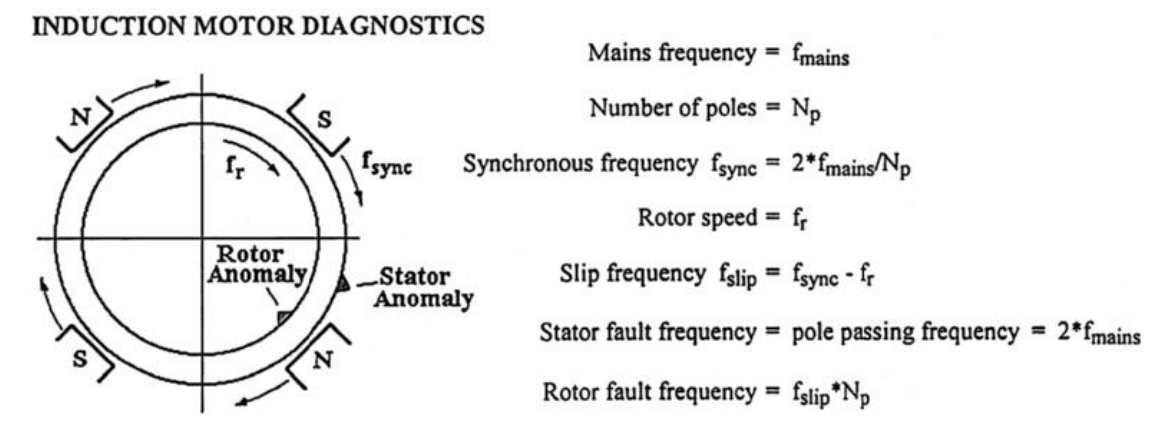
\includegraphics[scale=.35]{referencial/img/fault_freq_randall_p55.png}
    \end{center}
    \fonte{.} 
    \label{fig:}
\end{figure}


\begin{figure}[H]
    \caption{.}
    \begin{center}
        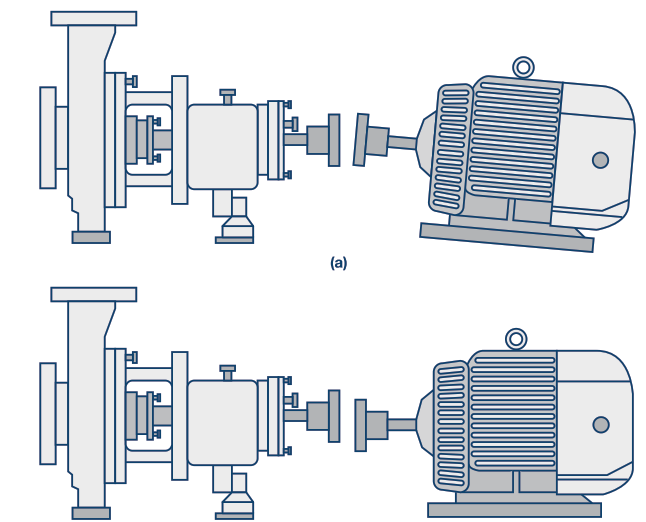
\includegraphics[scale=.45]{referencial/img/misadraw_analog_p2.png}
    \end{center}
    \fonte{.} 
    \label{fig:}
\end{figure}


\begin{figure}[H]
    \caption{.}
    \begin{center}
        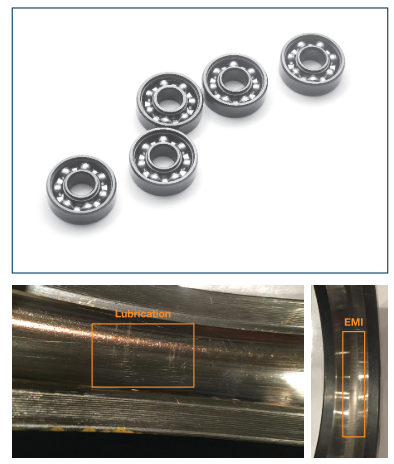
\includegraphics[scale=.5]{referencial/img/bearing_analog_p3.png}
    \end{center}
    \fonte{.} 
    \label{fig:}
\end{figure}

%++++++++++++++++++++++++++++++++++++++++++++++++++++++++++++++++
% 
%++++++++++++++++++++++++++++++++++++++++++++++++++++++++++++++++

\section{Análise de Vibração}\label{sec:}

Fazer:
\begin{itemize}
    \item breve esclarecimento entre os sinais amostrados e o espectro
    \item explicação sobre a amostragem nesses casos
\end{itemize}

\begin{figure}[H]
    \caption{.}
    \begin{center}
        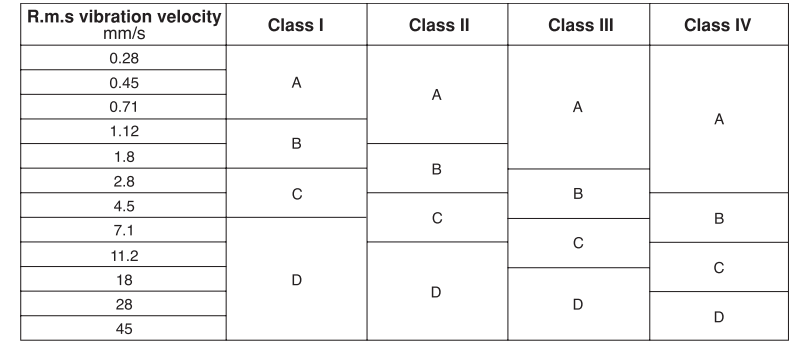
\includegraphics[scale=.5]{referencial/img/iso10816-1_randall_p146.png}
    \end{center}
    \fonte{.} 
    \label{fig:}
\end{figure}

\begin{figure}[H]
    \caption{.}
    \begin{center}
        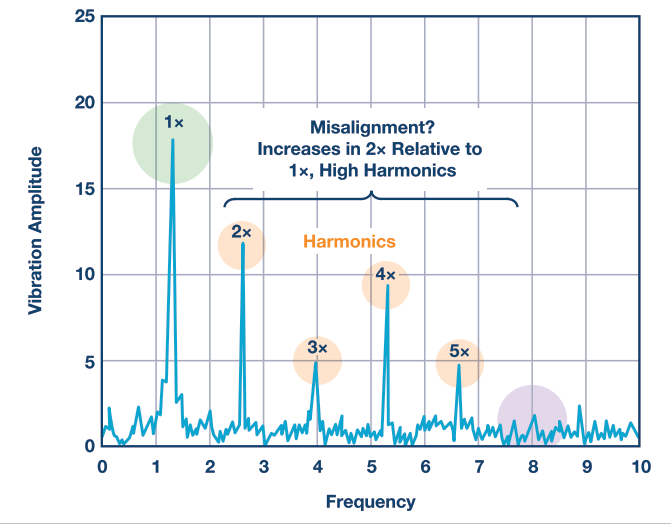
\includegraphics[scale=.4]{referencial/img/misa_analog_p2.png}
    \end{center}
    \fonte{.} 
    \label{fig:}
\end{figure}

\begin{figure}[H]
    \caption{.}
    \begin{center}
        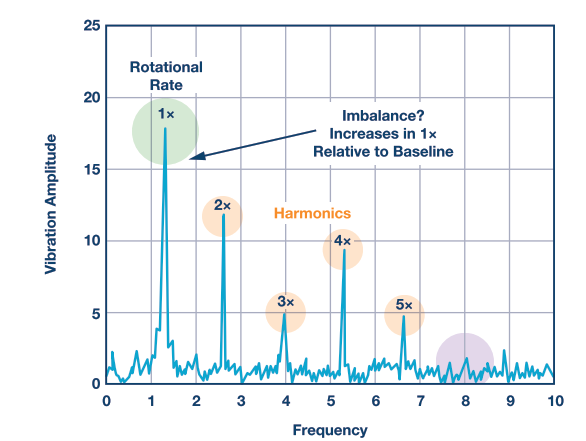
\includegraphics[scale=.5]{referencial/img/imbalance_analog_p2.png}
    \end{center}
    \fonte{.} 
    \label{fig:}
\end{figure}



%++++++++++++++++++++++++++++++++++++++++++++++++++++++++++++++++
% 
%++++++++++++++++++++++++++++++++++++++++++++++++++++++++++++++++

\section{Análise de Corrente Elétrica }\label{sec:}

ACHAR ALGO
aceito dicas :)

% \begin{figure}[H]
%     \caption{.}
%     \begin{center}
%         \includegraphics[scale=.5]{referencial/img/}
%     \end{center}
%     \fonte{.} 
%     \label{fig:}
% \end{figure}




%++++++++++++++++++++++++++++++++++++++++++++++++++++++++++++++++
% 
%++++++++++++++++++++++++++++++++++++++++++++++++++++++++++++++++

\section{Sistemas de Detecção de Falhas}\label{sec:}

\begin{figure}[H]
    \caption{.}
    \begin{center}
        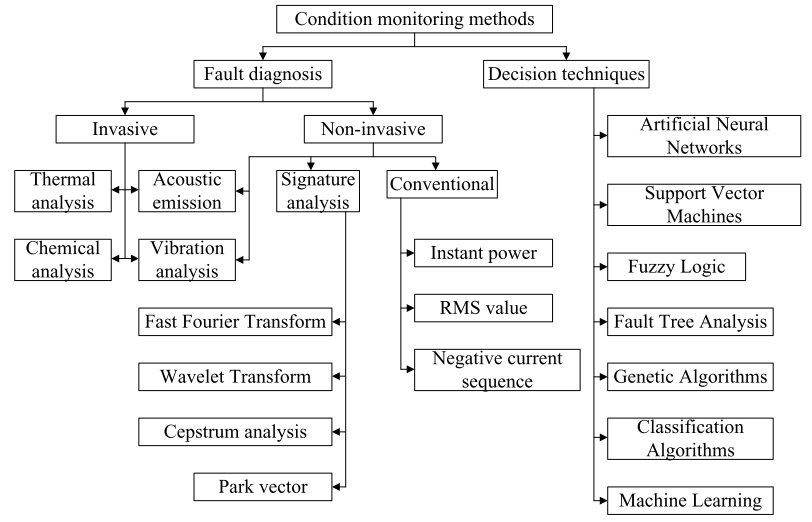
\includegraphics[scale=.5]{referencial/img/monitoring_methods_rilski_p78.png}
    \end{center}
    \fonte{.} 
    \label{fig:}
\end{figure}

%++++++++++++++++++++++++++++++++++++++++++++++++++++++++++++++++
% 
%++++++++++++++++++++++++++++++++++++++++++++++++++++++++++++++++

\section{Técnicas Modernas de Processamento de Sinais}\label{sec:}



%----------------------------------------------------------------
% 
%----------------------------------------------------------------

\subsection{RNA}

\begin{figure}[H]
    \caption{.}
    \begin{center}
        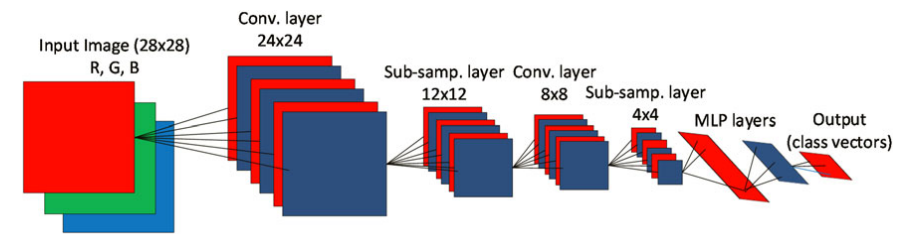
\includegraphics[scale=.4]{referencial/img/cnn_image_ince_p5.png}
    \end{center}
    \fonte{.} 
    \label{fig:}
\end{figure}


%----------------------------------------------------------------
% 
%----------------------------------------------------------------

\subsection{ICA}

% \begin{figure}[H]
%     \caption{.}
%     \begin{center}
%         \includegraphics[scale=.5]{referencial/img/}
%     \end{center}
%     \fonte{.} 
%     \label{fig:}
% \end{figure}


%----------------------------------------------------------------
% 
%----------------------------------------------------------------

\subsection{T-SNE}

\begin{figure}[H]
    \caption{.}
    \begin{center}
        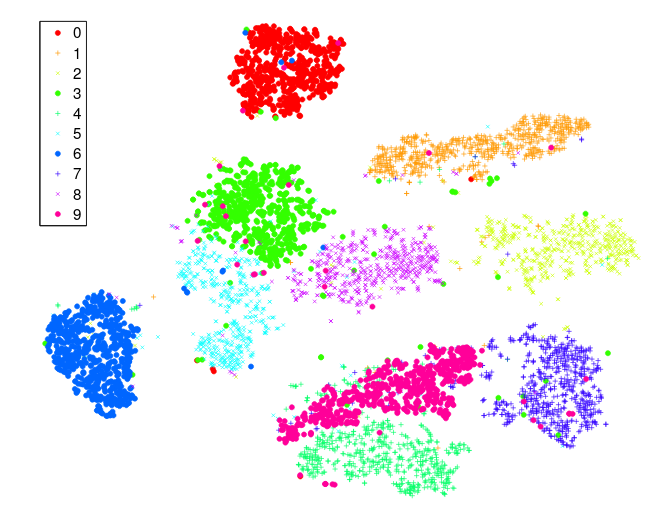
\includegraphics[scale=.45]{referencial/img/t-sne_matten_p2590.png}
    \end{center}
    \fonte{.} 
    \label{fig:}
\end{figure}

%----------------------------------------------------------------
% 
%----------------------------------------------------------------

\subsection{K-Means}

\begin{figure}[H]
    \caption{.}
    \begin{center}
        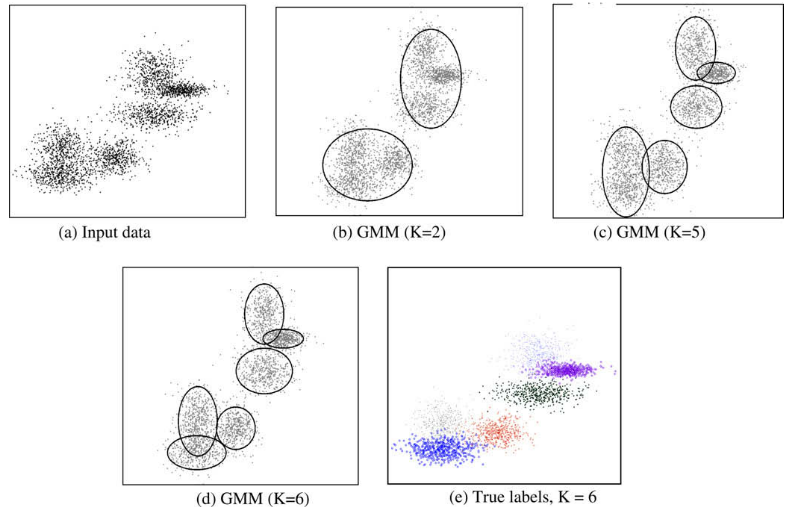
\includegraphics[scale=.5]{referencial/img/k-means_jain_p7.png}
    \end{center}
    \fonte{.} 
    \label{fig:}
\end{figure}


%++++++++++++++++++++++++++++++++++++++++++++++++++++++++++++++++
% 
%++++++++++++++++++++++++++++++++++++++++++++++++++++++++++++++++

\section{Estado da Arte}


%----------------------------------------------------------------
% 
%----------------------------------------------------------------

\subsection{RNA}

\begin{figure}[H]
    \caption{.}
    \begin{center}
        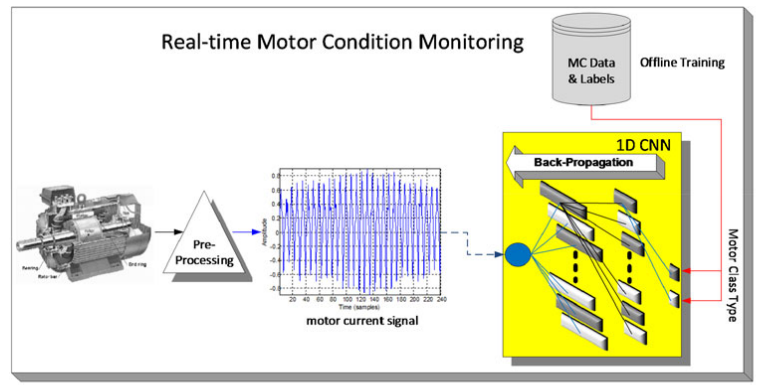
\includegraphics[scale=.45]{referencial/img/cnn_ince_p2.png}
    \end{center}
    \fonte{.} 
    \label{fig:}
\end{figure}

\begin{figure}[H]
    \caption{.}
    \begin{center}
        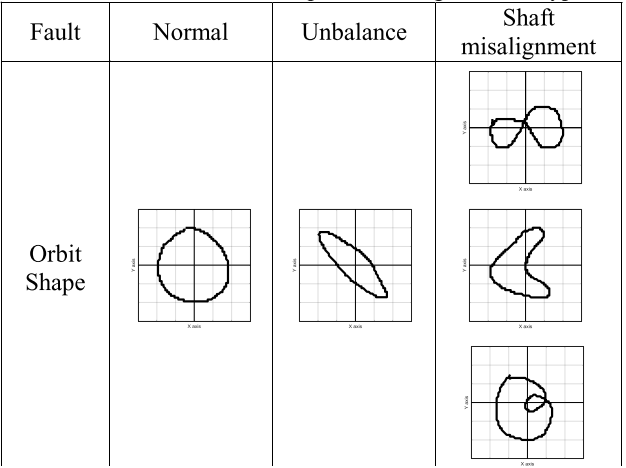
\includegraphics[scale=.45]{referencial/img/orbit_jeong_p3.png}
    \end{center}
    \fonte{.} 
    \label{fig:}
\end{figure}


%----------------------------------------------------------------
% 
%----------------------------------------------------------------

\subsection{ICA e PCA}

\begin{figure}[H]
    \caption{.}
    \begin{center}
        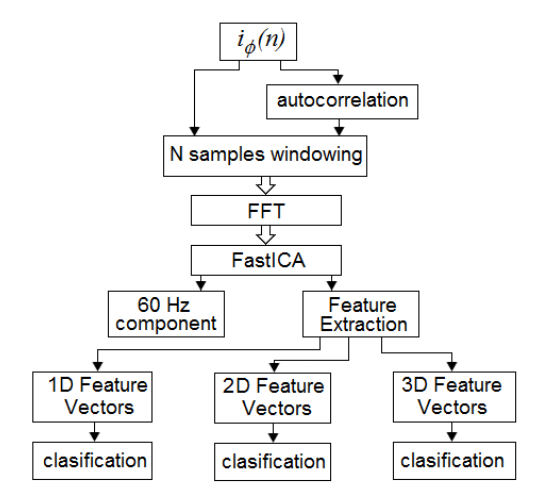
\includegraphics[scale=.5]{referencial/img/ica_bracamonte_p4.png}
    \end{center}
    \fonte{.} 
    \label{fig:}
\end{figure}